\documentclass[11pt]{article}

% EMNLP 2025 / ACL Rolling Review submission.
% Use the [review] option to enable line numbers for anonymous review.
% For camera-ready, switch to \usepackage[]{acl} (no [review]).
\usepackage[review]{acl}

\usepackage{times}
\usepackage{latexsym}
\usepackage[T1]{fontenc}
\usepackage[utf8]{inputenc}
\usepackage{microtype}
\usepackage{inconsolata}

\usepackage{hyperref}
\usepackage{url}
\usepackage{booktabs}
\usepackage{amsfonts}
\usepackage{amsmath}
\usepackage{nicefrac}
\usepackage{graphicx}
\usepackage{xcolor}
\usepackage{float}
\usepackage{caption}
\usepackage{multirow}
% \usepackage{subcaption}
\graphicspath{{figures/}}
\newcommand{\note}[1]{\textcolor{blue}{{#1}}}

\title{Knowing When You Don't Know:\\Separating Access Failures from Knowledge Gaps for Closed-Book Hallucination Mitigation}

\author{Anonymous ACL submission}

\begin{document}

\maketitle

\begin{abstract}
Small language models in closed-book QA hallucinate confidently because they cannot distinguish known facts from forgotten ones. We frame this failure as two distinct causes---\emph{access failures} (facts in parameters but not retrieved) and \emph{knowledge gaps} (facts absent)---and propose a pipeline targeting each. For access failures, Chain-of-Thought distillation from a 235B teacher under an ``internalized knowledge'' constraint recovers a 5.4-point EM gain on HotPotQA. For knowledge gaps, we label hallucinated training examples as ``I don't know'' and fine-tune under a class-balanced abstention objective, then refine with Reinforcement Learning from Verifier Feedback (RLVF). RLVF answers $+5$ percentage points more questions than the supervised model while \emph{raising} abstention precision to $97.84\%$; the full pipeline cuts confident hallucinations by $59\%$. As a byproduct, fine-tuning unlocks unsupervised uncertainty estimation: RAUQ and Semantic Entropy reach AUROC $0.86$ versus chance-level $0.43$--$0.51$ on the base model, a $+0.35$ gain over the P(true) baseline \citep{kadavath2022language}.
\end{abstract}

\section{Introduction}
Large Language Models (LLMs) frequently suffer from \emph{hallucination} in closed-book settings, generating plausible but factually incorrect assertions \cite{ji2023survey}. This issue is particularly acute in Small Language Models (SLMs), which often lack the capacity to distinguish between what they know and what they have forgotten. This unreliability creates a critical barrier for deployment in safety-critical or privacy-constrained environments where Retrieval-Augmented Generation (RAG) is not feasible.

We frame closed-book hallucination as arising from two distinct failure modes that require separate interventions. The first is an \emph{access failure}: the relevant fact is stored in the model's parameters, but the model cannot reliably surface it under standard decoding \cite{kadavath2022language}. The second is a \emph{knowledge gap}: the fact is simply not in the model's parameters, and any direct answer will be a guess. Treating these symmetrically (e.g., forcing the model to always answer) encourages confident hallucination on the second case; teaching it to always abstain wastes capability on the first.

Our pipeline targets each failure mode separately. To recover from access failures, we apply \textbf{Chain-of-Thought (CoT) Distillation} from a much larger teacher to unlock latent parametric knowledge through step-by-step recall. To handle genuine knowledge gaps, we apply \textbf{Abstention-Aware Fine-Tuning} followed by \textbf{Reinforcement Learning from Verifier Feedback (RLVF)}, which teaches the model to refuse rather than fabricate. We instantiate the pipeline on Qwen2.5-7B-Instruct.

Our experiments on HotPotQA validate this two-pronged approach. CoT distillation improves Exact Match accuracy from 18.86\% to 24.31\%, significantly outperforming standard SFT. Abstention-Aware Fine-Tuning achieves 97.5\% precision in detecting knowledge boundaries and cuts the rate of confident errors by more than half relative to the baseline. RLVF then provides a verifier-grounded mechanism for tuning the risk--coverage trade-off: it raises the answer rate by $5$ percentage points while \emph{improving} abstention precision to 97.84\%, the highest of any model in our evaluation. Together the supervised and RL stages cover two complementary deployment regimes: a conservative supervised model for safety-critical use and a coverage-oriented RL-tuned model for general assistance, both substantially safer than the baseline. As a byproduct, the same fine-tuning that produces native abstention behavior also turns the existing unsupervised uncertainty estimators of \citet{vazhentsev2025rauq} and \citet{Farquhar2024Detecting} from random ($\text{AUROC} = 0.43$) to predictive (up to $0.86$); on the same inputs, the P(true) self-evaluation baseline of \citet{kadavath2022language} stays at chance.

\paragraph{Contributions.} We make four contributions:
\begin{enumerate}
\item A \textbf{two-cause framing} of closed-book hallucination (access failure vs.\ knowledge gap) and a pipeline whose components map onto these causes one-to-one.
\item An \textbf{internalized-knowledge CoT distillation} recipe in which a 235B teacher generates rationales constrained to read as direct recall, with a validator that rejects citation-style traces. This recovers a 5.4-point absolute EM gain on HotPotQA under closed-book inference.
\item An \textbf{abstention-aware training pipeline} comprising (i) a knowledge-boundary mapping procedure that converts hallucinated training examples into ``I don't know'' supervision under an 80/20 class balance, and (ii) an RLVF stage whose reward combines a DeBERTa NLI verifier (open-book at training, closed-book at inference) with a token-level entropy confidence term. Together these cut confident hallucinations by up to 59\% relative to the base model.
\item An \textbf{evaluation in standard selective-prediction terms} (AUROC, AURC, Expected Calibration Error, Risk@Coverage). We show that the standard P(true) self-evaluation baseline of \citet{kadavath2022language} is at chance ($\text{AUROC} \approx 0.51$) on closed-book HotPotQA for both the base and fine-tuned model, while RAUQ \cite{vazhentsev2025rauq} and Semantic Entropy \cite{Farquhar2024Detecting}, when paired with our fine-tuned checkpoints, reach AUROC up to $0.86$, a $+0.35$ absolute gain over P(true). The same uncertainty estimators are anti-informative ($\text{AUROC} = 0.43$) on the un-fine-tuned base model, so the gain is attributable to the fine-tuning, not to the choice of estimator. Unsupervised Semantic Entropy is additionally an effective post-hoc filter, raising selective F1 from 0.50 to 0.70 at 50\% rejection.
\end{enumerate}

\section{Related Work}

\textbf{Hallucination in LLMs}: Hallucination refers to the generation of text that is nonsensical or unfaithful to the provided source or established world knowledge \cite{ji2023survey}. In closed-book settings, where models rely on parametric memory, hallucinations often stem from the model's inability to accurately assess the boundaries of its own knowledge \cite{kadavath2022language}. While larger models exhibit emergent self-calibration, Small Language Models (SLMs) are particularly prone to confident errors, necessitating explicit intervention strategies.

\textbf{Reasoning Distillation}: Chain-of-Thought (CoT) prompting significantly enhances LLM reasoning but typically requires large model scales (>100B parameters) to be effective. To transfer this capability to smaller models, \citet{li2023cotdistill} and \citet{ho2023largelanguagemodelsreasoning} proposed CoT distillation, where a student model is fine-tuned on reasoning traces generated by a large teacher. Our work extends this by imposing an \emph{internalized-knowledge} constraint on the teacher, ensuring the distilled reasoning relies on facts the student can plausibly retrieve from its own weights rather than external context.

\textbf{Abstention and Uncertainty}: Teaching models to say ``I don't know'' is a classic problem in reliable QA \citep{rajpurkar2018know}. Recent work splits into two families. \emph{Refusal-aware training} fine-tunes models to abstain on questions outside their knowledge boundary; R-Tuning \citep{zhang2024rtuning} and the self-evaluation framework of \citet{kadavath2022language} are the closest prior abstention baselines, the latter giving the P(true) signal we compare against. \emph{Unsupervised uncertainty estimation} instead derives a confidence score post-hoc from generation statistics; recent approaches include Semantic Entropy over generation clusters \citep{Farquhar2024Detecting}, attention-pattern-based methods such as RAUQ \citep{vazhentsev2025rauq}, and verbalized uncertainty \citep{lin2022teaching}. We combine both: knowledge-boundary-aware supervised fine-tuning followed by NLI-grounded RL (RLVF), and we then evaluate the resulting models with RAUQ, Semantic Entropy, and P(true) head-to-head.

\section{Approach}

Our pipeline is a sequence of five models. We use Qwen2.5-7B-Instruct \citep{qwen2025qwen25technicalreport} throughout as the policy backbone; each fine-tuned variant is a LoRA / QLoRA adapter trained on top of it. Two of the five are baselines (out-of-the-box and vanilla SFT), and three are our methods (CoT distillation, abstention SFT, and verifier-based RL).

\begin{itemize}
\item \textbf{Qwen2.5-Instruct} (baseline): the base model used out of the box.
\item \textbf{Qwen2.5-SFT} (baseline): LoRA fine-tuned on 10{,}000 question--answer pairs from HotPotQA.
\item \textbf{Qwen2.5-FCoT} (\emph{ours}): fine-tuned on Dataset B (Section~\ref{sec:finetune-cot}) to produce an internalized-knowledge rationale before answering.
\item \textbf{Qwen2.5-Abstain} (\emph{ours}): QLoRA fine-tuned on the answer / abstention pairs in Dataset C (Section~\ref{sec:abstension}).
\item \textbf{Qwen2.5-RLVF} (\emph{ours}): Qwen2.5-Abstain further trained with policy-gradient RL against a verifier-based reward (Section~\ref{sec:rlvf}).
\end{itemize}

\subsection{Finetune-CoT}\label{sec:finetune-cot}

To enable multi-step reasoning in the student model, we adopt the Fine-tune-CoT framework \cite{ho2023largelanguagemodelsreasoning}, which transfers reasoning ability from a large teacher to a smaller student by fine-tuning the student on rationales produced by the teacher. The standard pipeline has three stages: (1) prompting the teacher to generate step-by-step rationales, (2) curating the data by filtering samples whose final answer disagrees with the ground truth, and (3) fine-tuning the student on the validated traces.

We adapt the generation and curation stages to produce what we call an \emph{internalized-knowledge} dataset (Dataset B). By ``internalized knowledge'' we mean reasoning that is phrased as direct recall from the model's own parameters rather than as citation of an external passage, e.g., ``Arthur's Magazine was first published in 1844'' rather than ``the passage states that Arthur's Magazine was first published in 1844.'' This distinction matters because the student is deployed closed-book, so any habit of referring to ``the passage'' at training time produces incoherent outputs at inference time.

To produce this dataset, we use Qwen3-235B as the teacher and provide it with the HotPotQA supporting paragraphs as context to suppress its own hallucinations. We then prompt it to frame its rationale as a step-by-step recall of facts and explicitly forbid citation markers such as ``according to the passage.'' A validation loop rejects samples whose final answer is wrong (as in standard Fine-tune-CoT) and additionally rejects samples containing forbidden citation phrases, enforcing the internalized-knowledge style.

\subsection{Abstention-Aware Fine-Tuning}\label{sec:abstension}

To handle questions for which the model genuinely lacks the relevant knowledge, we fine-tune the model to output an explicit refusal (``I don't know'') rather than guess. Forcing the model to answer every query encourages hallucination on out-of-distribution facts; abstention-aware fine-tuning instead calibrates the model's behavior to its actual competence.

We first aimed to map the \emph{knowledge boundary} of Qwen2.5: the partition of HotPotQA training examples into those the model can answer from its own parameters and those on which it hallucinates. We hypothesize that if Qwen2.5-FCoT generates an incorrect answer for a training example $x$ under closed-book inference, that example lies outside the model's knowledge boundary and is hallucination-prone. We performed closed-book inference on the first $N=40{,}000$ examples of the HotPotQA training set. For every example, we compared the model's predicted answer $\hat{y}$ against the ground truth $y$ using Exact Match (EM) scoring. This effectively partitioned our training data into two sets: 
\begin{itemize}
    \item \textbf{Correct set} ($S_{\text{correct}}$): samples where the model's parametric knowledge sufficed ($\text{EM}(\hat{y}, y) = 1$).
    \item \textbf{Hallucination set} ($S_{\text{hallucination}}$): samples where the model produced a confident but incorrect answer ($\text{EM}(\hat{y}, y) = 0$).
\end{itemize}

Using this partition, we constructed a supervised fine-tuning dataset (Dataset C) that reinforces known knowledge while penalizing hallucinations. For examples in $S_{\text{hallucination}}$ we replaced the ground-truth answer with ``I don't know,'' and for examples in $S_{\text{correct}}$ we retained the original answer. A naive version of this objective is degenerate: if every hard question is relabeled to ``I don't know,'' the model can drive its loss to zero by always refusing, a failure mode we refer to as the \emph{laziness collapse}. To prevent this, we enforced an 80/20 class balance by randomly sampling 8{,}000 examples from $S_{\text{correct}}$ and 2{,}000 from $S_{\text{hallucination}}$, yielding a final 10{,}000-example dataset. We then fine-tuned Qwen2.5-Instruct with QLoRA on this mixture.

\subsection{Reinforcement Learning from Verifier Feedback}\label{sec:rlvf}

To refine the abstention boundary learned during supervised fine-tuning, we further train Qwen2.5-Abstain with policy-gradient RL against a reward derived from a verifier and from the model's own confidence. Although the policy is queried closed-book at training time, the verifier itself is \emph{not}: it is given the HotPotQA supporting paragraphs, so the reward measures semantic alignment with grounded evidence rather than exact-match against a single gold string.

\paragraph{FactualityVerifier.} We use a DeBERTa-based NLI model \cite{he2021deberta,he2021debertav3} that takes a premise and a hypothesis and returns class probabilities over $\{\text{entailment}, \text{neutral}, \text{contradiction}\}$. For each training example we concatenate the supporting paragraph titles and sentences from HotPotQA \cite{yang2018hotpotqadatasetdiverseexplainable} into a single premise, treat the model's generated answer as the hypothesis, and read off the entailment and contradiction probabilities $p_{\text{ent}}$ and $p_{\text{cont}}$. We define a grounded factuality score
\[
f = p_{\text{ent}} - p_{\text{cont}} \in [-1, 1],
\]
so that $f > 0$ corresponds to answers that the supporting paragraphs entail and $f < 0$ to answers they contradict. Thus RLVF optimizes semantic factuality against the verifier rather than string-level agreement with a gold label.

\paragraph{Confidence Term.}
We reward the policy for being correct \emph{confidently}, with confidence defined as the complement of mean per-token entropy normalized by the maximum possible entropy:
\[
\text{conf} = 1 - \frac{H_{\text{avg}}}{H_{\max}} \in [0, 1],
\]
where $H_{\text{avg}} = \frac{1}{T}\sum_{t} H(p_t)$ is the mean Shannon entropy of the policy's next-token distribution $p_t$ over the $T$ generated tokens, and $H_{\max} = \log|V|$. We use this token-level form (rather than the semantic-entropy form of \citet{Farquhar2024Detecting}, which inspired it) because it can be computed cheaply on-policy during RL rollouts. As the reward function below specifies, confidence amplifies reward only when factuality is positive, preventing the policy from being rewarded for confidently wrong answers.

\paragraph{Abstention Detection.}
We do not detect abstentions by string matching, which is brittle to paraphrases (``I'm not sure,'' ``I don't have that information,'' etc.). Instead, our \emph{AbstentionClassifier} reuses the NLI verifier: it treats the generated answer as a premise and a canonical abstention statement (``The respondent does not know the answer'') as the hypothesis, and flags the answer as an abstention if the entailment probability exceeds a fixed threshold. This is analogous in spirit to prior work on verbalized uncertainty \cite{lin2022teaching}. Detected abstentions receive a fixed reward of $-1.0$, making refusal mildly costly but strictly cheaper than a contradiction.

\paragraph{Reward Function.}
For non-abstaining outputs, the reward depends only on verifier factuality and confidence:
\[
R =
\begin{cases}
10\, f (\lambda_{\text{base}} + \lambda_{\text{conf}}\cdot\text{conf}) & f \ge 0, \\
5\, f (\lambda_{\text{base}} + \lambda_{\text{conf}}\cdot\text{conf})  & f < 0.
\end{cases}
\]
$\lambda_{\text{base}}$ and $\lambda_{\text{conf}}$ are fixed scalars controlling the reward floor and the maximum confidence bonus. The asymmetric $10\times$/$5\times$ scaling rewards grounded answers more strongly than it punishes contradictions of equal magnitude, which biases the policy toward attempting answers and counterbalances the strong incentive (from the conservative SFT initialization) to default to abstention. The choice to ground the reward in the NLI verifier rather than Exact Match avoids penalizing valid paraphrases of the gold answer \cite{ji2023survey}, and the warm-start from Qwen2.5-Abstain (rather than from the base) gives the RL stage a pre-existing abstention boundary to refine, which we found necessary for stable early optimization \cite{ho2023largelanguagemodelsreasoning}.

\subsection{Discrete Semantic Entropy}\label{sec:se-method}

We use Discrete Semantic Entropy (SE) \cite{Farquhar2024Detecting} as a post-hoc, training-free signal for residual hallucinations after the abstention pipeline. We adopt the discrete (black-box) form rather than RAUQ \cite{vazhentsev2025rauq} because the inference API for our larger model does not expose internal attention weights. For each question $x$ we draw $M=10$ stochastic generations and cluster them by bidirectional NLI entailment (\texttt{microsoft/deberta-large-mnli}). The probability of each semantic cluster $C$ is approximated by Monte Carlo:
\begin{equation}
P(C \mid x) \approx \frac{1}{M} \sum_{i=1}^M \mathbb{I}(s_i \in C),
\end{equation}
and the total uncertainty is the entropy over clusters,
$H(x) = -\sum_{C} P(C \mid x) \log P(C \mid x).$
We use $H(x)$ as a per-question uncertainty score, sort the validation set in descending order, and rank-reject the top-$k$ most uncertain samples to produce rejection curves (Section~\ref{sec:results-se}).

\section{Experiments}
\subsection{Data}
We use the training and validation splits of the HotPotQA \cite{yang2018hotpotqadatasetdiverseexplainable} distractor dataset. The distractor setting has question-answer pairs with ten paragraphs as context, two of which are relevant to answering the question. Since we ran our tests in a closed-book setting, we discarded all ten context paragraphs for our finetuning, RL, and evaluation methods. We define 3 training datasets:

\textbf{Dataset A1/A2: } The first and second 10,000 question-answer pairs of HotPotQA (distractor setting, train split), respectively. 

\textbf{Dataset B:} The first 10,000 HotPotQA distractor/train examples augmented with teacher-generated rationales under our internalized-knowledge constraint (Section~\ref{sec:finetune-cot}). A representative entry:
\begin{itemize}
    \item \textbf{Q:} Which magazine was started first, Arthur's Magazine or First for Women?
    \item \textbf{R:} \emph{Step 1}: The question asks ... \emph{Step 2}: Arthur's Magazine was published starting in 1844 \dots \emph{Step 3}: Since 1844 is earlier than the 1980s, the answer is Arthur's Magazine.\footnote{Reasoning trace abbreviated for space.}
    \item \textbf{A:} Arthur's Magazine.
\end{itemize}

\textbf{Dataset C:} 10,000 question--answer or question--abstention pairs sampled from the first 40,000 HotPotQA distractor/train examples (Section~\ref{sec:abstension}). A representative abstention entry:
\begin{itemize}
    \item \textbf{Q:} Who wrote the 1971 drama which stars the winner of the 1997 BAFTA Fellowship?
    \item \textbf{A:} I don't know.
\end{itemize}

\subsection{Evaluation method}
We measure answering quality with Exact Match (EM) and token-level F1 between the gold answer and the model's prediction. For abstention models, we report two additional quantities: the \emph{abstention rate}, defined as the fraction of validation questions for which the model output an ``I don't know''-style response (as judged by the AbstentionClassifier), and the \emph{selective EM/F1}, defined as EM/F1 computed only on the answered subset.

To assess whether high-uncertainty samples are also high-error samples, we additionally compute two unsupervised uncertainty signals on each generation: RAUQ \cite{vazhentsev2025rauq}, which aggregates attention-weight patterns across heads to score how anomalous a generation is, and Semantic Entropy (SE) \cite{Farquhar2024Detecting}, defined below in Section~\ref{sec:se-method}. We sort model responses by each uncertainty score and report \emph{rejection curves}: EM/F1 on the retained subset as a function of the fraction of most-uncertain samples discarded. These curves serve as a non-parametric upper bound on what a perfectly calibrated abstention policy could achieve.

\subsection{Experimental details}

\paragraph{Models and infrastructure.}
All rows in the main results table use \textbf{Qwen2.5-7B-Instruct} (bfloat16) as the policy backbone; SFT, FCoT, Abstain, and RLVF are LoRA / QLoRA adapters (4-bit NF4 base, FP16 adapters) on top of it. A separate scaled re-implementation of CoT distillation and abstention SFT (with the full 80K HotPotQA training set rather than the 10K subset) was performed on \textbf{Qwen3-8B} on a higher-throughput platform that did not host a Qwen2.5 checkpoint. We verified on the closed-book validation split that Qwen3-8B and Qwen2.5-7B agree on EM/F1 to within $\pm 1$ point on the same training data, but the Qwen3-8B re-runs are not reported in the main table to keep the comparison apples-to-apples across rows.

\paragraph{Training configuration.}
We applied LoRA ($r=16$, $\alpha=32$, dropout $0.05$) to all linear projection layers. Optimization used \texttt{adamw\_torch} with a cosine scheduler (3\% warmup) and an effective batch size of 16. All fine-tuning runs were one epoch. \textbf{Supervised baselines (SFT, FCoT, Abstain)} used learning rate $2{\times}10^{-4}$. SFT used standard chat formatting (max length 512) with user prompts masked from the loss. FCoT and Abstain used a \texttt{Question \#\#\# Rationale --> Answer} delimiter format (max length 2048) so the rationale and answer can be parsed deterministically at inference. Qwen2.5-SFT was trained on Dataset~A1, Qwen2.5-FCoT on Dataset~B, and Qwen2.5-Abstain on Dataset~C. \textbf{Qwen2.5-RLVF} was initialized from the Qwen2.5-Abstain checkpoint and trained with on-policy rollouts on Dataset~A2 at learning rate $1{\times}10^{-5}$ and weight decay $0.01$.

\paragraph{Inference.}
All evaluation was closed-book with greedy decoding. Standard (non-reasoning) models received a concise system prompt restricting outputs to short entities (max 50 tokens). Reasoning models were prompted with the \texttt{\#\#\#} delimiter to trigger a rationale (max 512 tokens) and the final answer was parsed from after \texttt{-->}.


\subsection{Results}

\begin{table*}[t]
\centering
\small
\caption{Main results on HotPotQA validation (distractor setting, closed-book; $N=7405$). EM and F1 are token-level percentages. Abs.\ Rate is the fraction of questions answered with an ``I don't know''-style refusal (judged by the AbstentionClassifier of Section~\ref{sec:rlvf}); Sel.\ EM/F1 are computed over the non-abstained subset; Avg.\ RAUQ is the mean per-question RAUQ uncertainty score. PaLM-62B is included as a larger-model closed-book reference point (from the RECITE paper); it is $\sim 9\times$ larger than our policy backbone.}
\label{tab:hotpotqa_comparison}
\begin{tabular}{lrrrrrr}
\toprule
\textbf{Model} & \textbf{EM} & \textbf{F1} & \textbf{Abs.\ Rate} & \textbf{Sel.\ EM} & \textbf{Sel.\ F1} & \textbf{Avg.\ RAUQ} \\
\midrule
\multicolumn{7}{l}{\emph{Our experiments ($N=7405$; Qwen2.5-7B-Instruct backbone)}} \\
\cmidrule(lr){1-7}
Qwen2.5-Instruct  & 18.86 & 27.02 & --     & --    & --    & 1.25 \\
Qwen2.5-SFT       & 21.94 & 31.41 & --     & --    & --    & 1.62 \\
Qwen2.5-FCoT      & \textbf{24.31} & 33.87 & --     & --    & --    & --   \\
Qwen2.5-Abstain   & 19.47 & 25.78 & 46.34  & 37.98 & 48.46 & 1.32 \\
Qwen2.5-RLVF      & 20.37 & 26.24 & 41.17  & 34.62 & 44.60 & 1.40 \\
\midrule
\multicolumn{7}{l}{\emph{Larger-model closed-book reference}} \\
\cmidrule(lr){1-7}
PaLM-62B   & 26.46 & 35.67 & N/A & N/A & N/A & N/A \\
\bottomrule
\end{tabular}
\end{table*}

\paragraph{Generation performance and error correction.}
Our fine-tuning experiments show clear improvements over the Qwen2.5-Instruct baseline across all metrics. As shown in Table~\ref{tab:model_performance}, FCoT achieves the highest Exact Match of 24.31\%, a 5.4-point absolute gain over the base model's 18.86\%. FCoT also corrects more baseline errors than plain SFT (697 vs.\ 477) at a comparable regression count (294 vs.\ 249), so the net gain is real. Strikingly, our $7$B FCoT essentially matches closed-book PaLM-62B (a model with $\sim 9\times$ more parameters), reaching $92\%$ of its EM ($24.31$ vs.\ $26.46$; Table~\ref{tab:hotpotqa_comparison}). The comparison is not strictly like-for-like (different architecture, different data), but it indicates that under closed-book reasoning, capacity is not the only path to performance: an internalized-knowledge CoT recipe can close most of the parameter-count gap.

\paragraph{Abstention precision and recall.}
Table~\ref{tab:abstention_analysis} reports precision and recall of each abstention model against four reference comparators (base, SFT, FCoT, and the ``Hardest'' subset of questions all three reference models answered incorrectly). Precision is the fraction of abstentions that correspond to questions the reference model got wrong (i.e., justified refusals); recall is the fraction of reference-model errors the abstention model successfully refused. Both abstention-trained variants achieve very high precision: \textbf{Qwen2.5-RLVF reaches 97.84\% precision against the base model, the highest of any model in our evaluation}, narrowly above the 97.49\% of Qwen2.5-Abstain. In other words, when our final model refuses, it is almost certainly right to do so.

\paragraph{Confident-error reduction across two operating points.}
EM penalizes wrong answers and abstentions identically and so hides the central effect we care about: how often the model emits a \emph{confident hallucination}, which we measure directly as $\text{attempted} \times (1 - \text{selective EM})$. The non-abstaining models all sit near 80\% (Instruct 81.14\%, SFT 78.06\%, FCoT 75.69\%) because they cannot refuse. Our abstention-trained models change this sharply at two operating points on the risk--coverage frontier (Figure~\ref{fig:rlhf_confusion_matrices}): \textbf{Qwen2.5-Abstain} (\emph{conservative}) answers 53.66\% of questions at 97.49\% abstention precision, leaving a confident-error rate of $\mathbf{33.28\%}$: a $\mathbf{59\%}$ relative reduction over the base model with EM almost unchanged ($18.86 \to 19.47$). \textbf{Qwen2.5-RLVF} (\emph{coverage-oriented}) answers $5$ more points of questions (58.83\%) while \emph{raising} abstention precision to $\mathbf{97.84\%}$ (the highest of any model in our evaluation) and keeping confident errors at $\mathbf{38.46\%}$, a $\mathbf{53\%}$ relative reduction.

\subsection{Selective Prediction Metrics}\label{sec:results-selective}

\begin{table*}[t]
\centering
\caption{Selective prediction on HotPotQA validation. Higher AUROC is better; lower AURC, Risk@k, and ECE are better. Computed by \texttt{analysis/compute\_selective\_metrics.py} from per-example prediction JSONs.}
\label{tab:selective-metrics}
\begin{tabular}{llrrrrrrr}
\toprule
\textbf{Model} & \textbf{Uncertainty} & $N$ & EM & F1 & AUROC $\uparrow$ & AURC $\downarrow$ & Risk@50 $\downarrow$ & ECE $\downarrow$ \\
\midrule
\multicolumn{9}{l}{\emph{Prior-method baseline: P(true), \citealp{kadavath2022language}}} \\
\cmidrule(lr){1-9}
Qwen2.5-Instruct & P(true) & 7405 & 0.182 & 0.262 & 0.508 & 0.819 & 0.810 & -- \\
Qwen2.5-SFT      & P(true) & 7405 & 0.209 & 0.302 & 0.502 & 0.794 & 0.785 & -- \\
\midrule
\multicolumn{9}{l}{\emph{Our methods}} \\
\cmidrule(lr){1-9}
Qwen2.5-Instruct & RAUQ    & 7405 & 0.182 & 0.262 & 0.431 & 0.807 & 0.865 & 0.523 \\
Qwen2.5-SFT      & RAUQ    & 7405 & 0.209 & 0.302 & \textbf{0.856} & \textbf{0.606} & \textbf{0.607} & 0.400 \\
Qwen2.5-RLVF     & SE      & 1000 & 0.232 & 0.320 & 0.826 & 0.580 & 0.588 & 0.480 \\
\bottomrule
\end{tabular}
\end{table*}

To put our results in standard selective-prediction terms, Table~\ref{tab:selective-metrics} reports AUROC of the uncertainty score against correctness (higher is better, $0.5$ = random), Area Under the Risk--Coverage curve (AURC; lower is better), risk at fixed coverage levels of 50\% and 80\% (lower is better), and Expected Calibration Error (ECE; lower is better, with 15 equal-frequency bins). We use RAUQ as the uncertainty score for greedy-decoded models and Semantic Entropy for the RLVF model under stochastic decoding. As a prior-method comparison, we additionally report the P(true) self-evaluation baseline of \citet{kadavath2022language}, in which the same model is asked ``Is the proposed answer correct?'' and the probability of \texttt{Yes} (renormalized over \{Yes, No\}) is taken as confidence.

\paragraph{Fine-tuning is the lever, not the estimator.}
P(true) is at chance on both the base model ($0.508$) and on Qwen2.5-SFT ($0.502$); the self-evaluation prompt does not depend on output structure and is unaffected by fine-tuning. RAUQ on the un-fine-tuned base is also uninformative, in fact anti-informative ($0.431$, below chance) because the base model frequently emits 1--3-token outputs on which attention-based confidence is degenerate. The same RAUQ estimator on the supervised fine-tuned model jumps to AUROC $0.856$; Semantic Entropy on the RLVF model reaches $0.826$. AURC drops from $0.79$--$0.82$ under P(true) to $0.58$--$0.61$ under our methods, and ECE drops by 10--12 points. The $+0.35$ absolute AUROC gain is therefore attributable to fine-tuning (which produces longer, more structured outputs) rather than to the choice of estimator; we view this as evidence for a \emph{fine-tuning-then-estimator} pipeline.

\subsection{Semantic-Entropy Rejection Curves}\label{sec:results-se}

\begin{figure*}[t]
    \centering
    \setlength{\abovecaptionskip}{2pt}
    \begin{minipage}{0.48\textwidth}
        \centering
        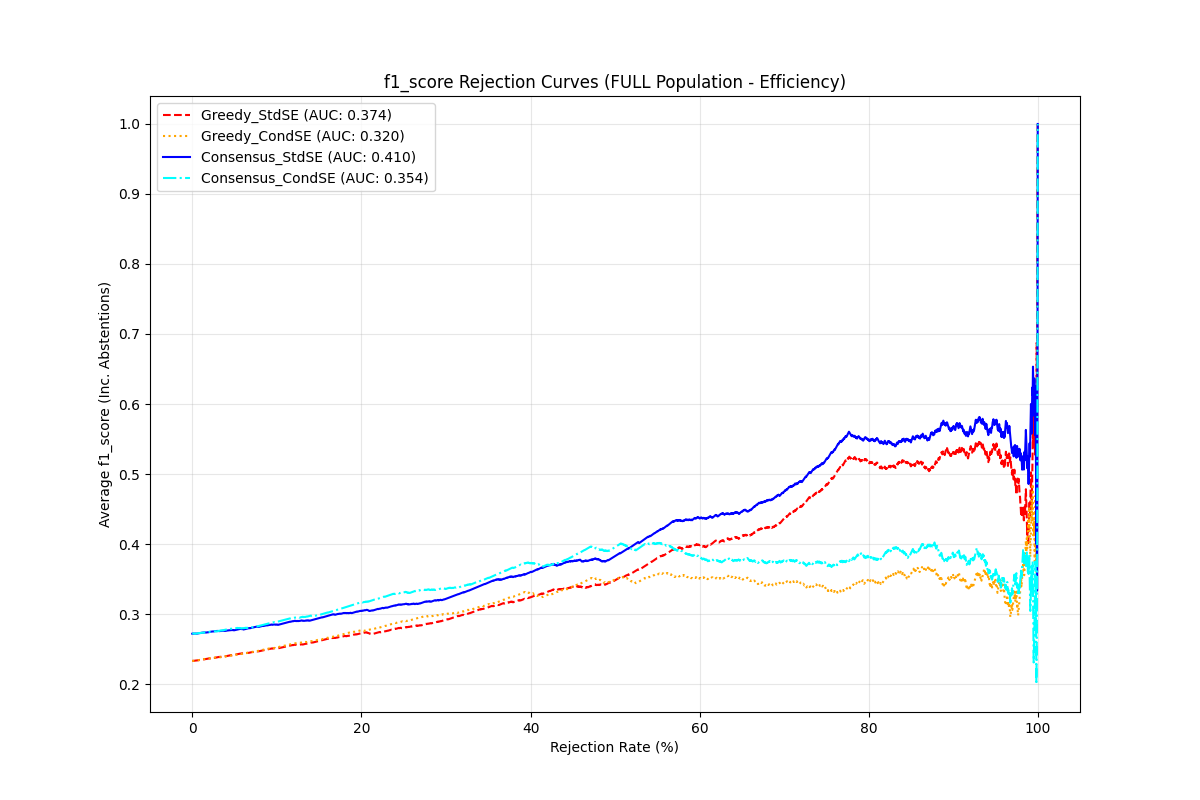
\includegraphics[height=5cm, keepaspectratio]{se_curves_full_f1_score.png}
        \caption*{Full Population (Efficiency)}
    \end{minipage}%
    \hfill
    \begin{minipage}{0.48\textwidth}
        \centering
        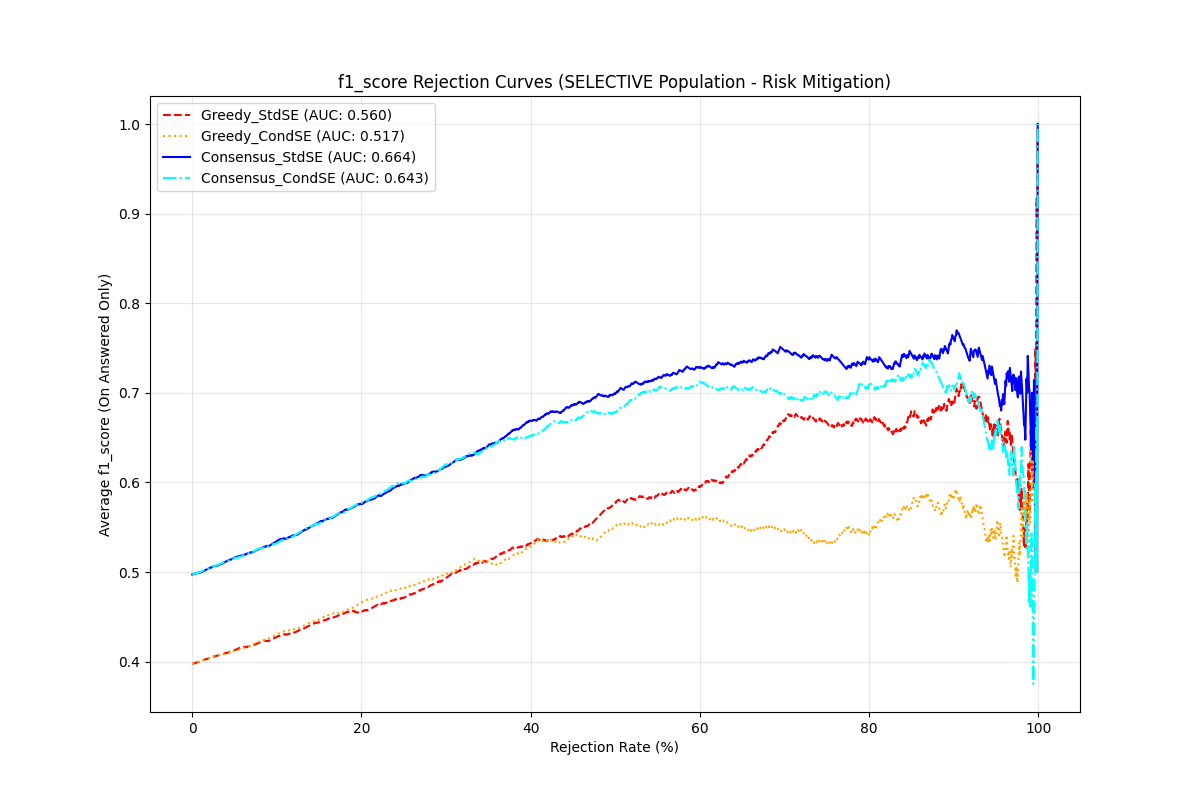
\includegraphics[height=5cm, keepaspectratio]{se_curves_selective_f1_score.png}
        \caption*{Selective Population (Risk Mitigation)}
    \end{minipage}
    \caption{F1 rejection curves: efficiency on the full dataset (left) vs.\ risk mitigation on answered questions (right). Both panels rank questions by Semantic Entropy and remove the top-$k$\%; Consensus dominates Greedy at every rejection rate, reaching selective F1 $0.70$ at 50\% rejection.}
    \label{fig:se_f1_curves}
\end{figure*}

Semantic Entropy is a strong proxy for correctness: correct answers cluster tightly around SE $\approx 0$ while incorrect answers have median SE $\approx 0.9$ (Appendix~\ref{app:se_dist}). It is also informative about the model's own refusals: both standard SE and conditional SE (which strips the ``I don't know'' cluster) are shifted higher for the model's abstained subset than for its answered subset, indicating the native abstention mechanism aligns with semantic uncertainty even when it does not perfectly separate the two distributions. Figure~\ref{fig:se_f1_curves} and Table~\ref{tab:se_rejection_f1} show the efficiency of using SE for post-hoc rejection. We compare a \emph{Greedy} strategy (confidence from the single most likely sequence) against a \emph{Consensus} strategy (marginalising probability mass over all sampled generations in the same semantic cluster). Consensus dominates Greedy at every rejection rate: at 0\% rejection it reaches selective F1 $0.50$ vs.\ Greedy's $0.40$, and at 50\% rejection it reaches selective F1 $\mathbf{0.70}$, confirming that aggregating semantic consistency across multiple samples is a more robust hallucination signal than a single-path decode.
\section{Analysis}

\subsection{Reasoning Trace: Qualitative Check}

Qualitative inspection of FCoT outputs (Appendix~\ref{app:qualitative}) confirms that the model learned the internalized-knowledge style; e.g., on ``Were Scott Derrickson and Ed Wood of the same nationality?,'' FCoT retrieves both nationalities from parameters and corrects the baseline's \emph{No} to \emph{yes} without ever referring to ``the passage.'' Regressions cluster into two modes. \textbf{Hallucination via reasoning}: step-by-step generation can induce false details (the model claims Rose McGowan was best known for \emph{Buffy the Vampire Slayer}, conflating two different actresses and shows, overriding the base model's correct \emph{Charmed} answer). \textbf{Granularity mismatch}: the trace can over-specify (deducing ``film director'' against the rigid gold ``director''); this is a limitation of Exact Match on reasoning outputs rather than of the model, and supports our decision to also report token-level F1.


\subsection{SFT vs.\ RLVF: Complementary Operating Points}

The two stages produce models with qualitatively different behaviour. On \emph{``What army did the namesake of the ship launched as the M\"unchen in 1930 fight in during the American Revolutionary War?''}, the supervised model abstains; RLVF answers \emph{Continental Army} (correct), recovering parametric knowledge the conservative model declines to commit to. On \emph{``What government position was held by the woman who portrayed Corliss Archer in \textit{Kiss and Tell}?''}, the supervised model again abstains; RLVF answers \emph{First Lady} (the correct answer is \emph{Chief of Protocol}), a confident error from the same reward shape that recovered the previous case. The two stages thus expose complementary operating points: the supervised model fits safety-critical deployments (97.5\% abstention precision, lowest confident-error rate), and the RL-tuned model fits general-assistant deployments (97.84\% abstention precision, $+5$-point coverage). Both come from the same pipeline and differ only in whether the abstention boundary is fixed by supervised labels or refined against a verifier reward; the RL stage's methodological contribution is the reward-shaped lever, which a sweep of the abstention penalty would let one move along.

\section{Conclusion}
We decomposed closed-book hallucination into access failures and knowledge gaps and built a pipeline that addresses each: CoT distillation (5.4-point EM gain), abstention-aware SFT (97.5\% abstention precision), and verifier-grounded RL (97.84\% abstention precision at $+5$ points of coverage). The supervised and RL stages expose two complementary operating points on the risk--coverage frontier and both cut confident hallucinations by up to 59\% over the base model. In standard selective-prediction terms, fine-tuning, not the choice of uncertainty estimator, lifts RAUQ and Semantic Entropy from chance to AUROC up to $0.86$, a $+0.35$ absolute gain over the P(true) self-evaluation baseline. Natural follow-ups include a hyperparameter sweep over the abstention penalty to densify the risk--coverage curve, and extension to open-book settings where the model must discriminate parametric knowledge from retrieved context.

\section*{Limitations}

\paragraph{Benchmark scope.} Our experiments are on HotPotQA distractor in a closed-book setting, a short-form English factoid benchmark over Wikipedia-derived text. Generalization to long-form, non-English, or domain-specialised QA is a natural extension and remains open.

\paragraph{Inference cost of Semantic Entropy.} Post-hoc SE filtering requires $M{=}10$ stochastic samples plus pairwise NLI clustering per question. This is an effective filter but multiplies inference compute over a single greedy decode; cheaper proxies (e.g., RAUQ as a pre-filter) are a useful direction.

\bibliographystyle{acl_natbib}
\bibliography{references}

\appendix

\section{Appendix}

\subsection{Qualitative Reasoning-Trace Examples}\label{app:qualitative}

Tables~\ref{tab:cot-success} and~\ref{tab:cot-failures} below give the full reasoning traces summarised in Section~5.1.

\begin{table}[H]
\centering
\small
\renewcommand{\arraystretch}{1.2}
\begin{tabular}{|p{0.45\linewidth}|p{0.5\linewidth}|}
\hline
\textbf{Context (Base Wrong $\rightarrow$ CoT Correct)} & \textbf{Generated Reasoning Trace} \\
\hline
\textbf{Q:} Were Scott Derrickson and Ed Wood of the same nationality? \newline
\textbf{Gold:} yes \newline
\textbf{Base Pred:} No (Wrong) \newline
\textbf{CoT Pred:} yes (Correct) &
Step 1: The question asks about the nationalities of Scott Derrickson and Ed Wood. \newline
Step 2: Scott Derrickson is an American film director\dots while Ed Wood was an American filmmaker\dots \newline
Step 3: Since both individuals were born and active in the United States\dots the answer is yes. \\
\hline
\end{tabular}
\caption{Example of successful internalized-knowledge retrieval by Qwen2.5-FCoT.}
\label{tab:cot-success}
\end{table}

\begin{table}[H]
\centering
\small
\renewcommand{\arraystretch}{1.2}
\begin{tabular}{|p{0.45\linewidth}|p{0.5\linewidth}|}
\hline
\textbf{Context (Base Correct $\rightarrow$ CoT Wrong)} & \textbf{Reasoning Trace Fault} \\
\hline
\multicolumn{2}{|c|}{\textbf{Failure Mode 1: Hallucination via reasoning}} \\
\hline
\textbf{Q:} What WB supernatural drama series was Jawbreaker star Rose McGowan best known for being in? \newline
\textbf{Gold/Base:} Charmed \newline
\textbf{CoT Pred:} Buffy the Vampire Slayer &
Step 2: Rose McGowan is best known for her role as Cordelia Chase in the WB supernatural drama series ``Buffy the Vampire Slayer.'' \newline
\textit{(Error: hallucinated role / show.)} \\
\hline
\multicolumn{2}{|c|}{\textbf{Failure Mode 2: Granularity mismatch}} \\
\hline
\textbf{Q:} What occupation do Chris Menges and Aram Avakian share? \newline
\textbf{Gold/Base:} Director \newline
\textbf{CoT Pred:} film director &
Step 3: Since both individuals are primarily recognized for directing films, their shared occupation is film director. \newline
\textit{(Error: trace too specific for gold label.)} \\
\hline
\end{tabular}
\caption{CoT failure modes (regression cases).}
\label{tab:cot-failures}
\end{table}

\subsection{Abstention Model vs. SE Analysis}\label{app:se_dist}

\begin{figure*}[t]
    \centering
    \setlength{\abovecaptionskip}{2pt}
    \begin{minipage}{0.32\textwidth}
        \centering
        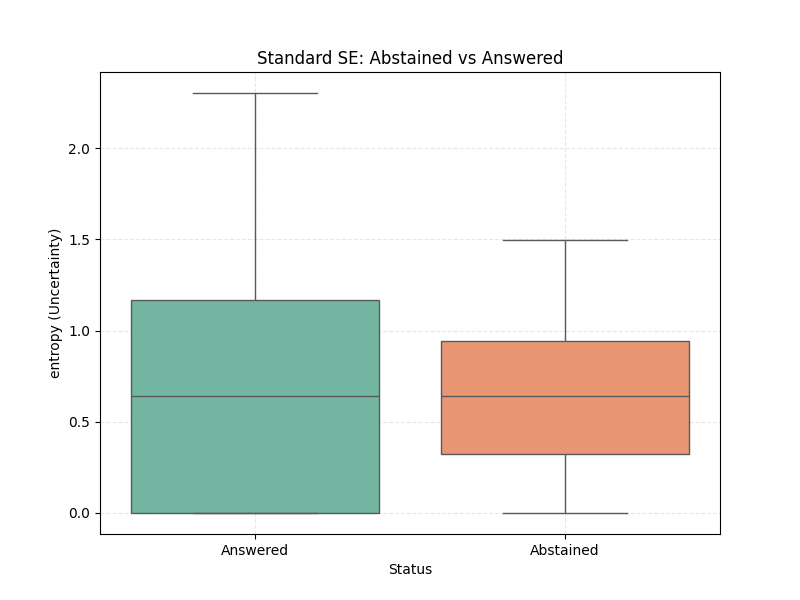
\includegraphics[height=3.5cm, keepaspectratio]{se_correlation_boxplot_std.png}
        \caption*{Std SE: Abstained vs.\ Answered}
    \end{minipage}%
    \hfill
    \begin{minipage}{0.32\textwidth}
        \centering
        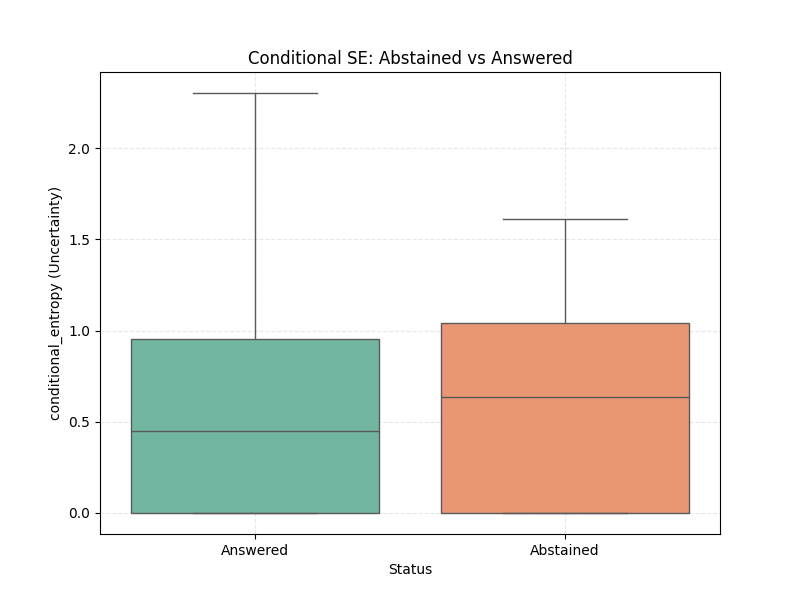
\includegraphics[height=3.5cm, keepaspectratio]{se_correlation_boxplot_cond.png}
        \caption*{Cond SE: Abstained vs.\ Answered}
    \end{minipage}%
    \hfill
    \begin{minipage}{0.32\textwidth}
        \centering
        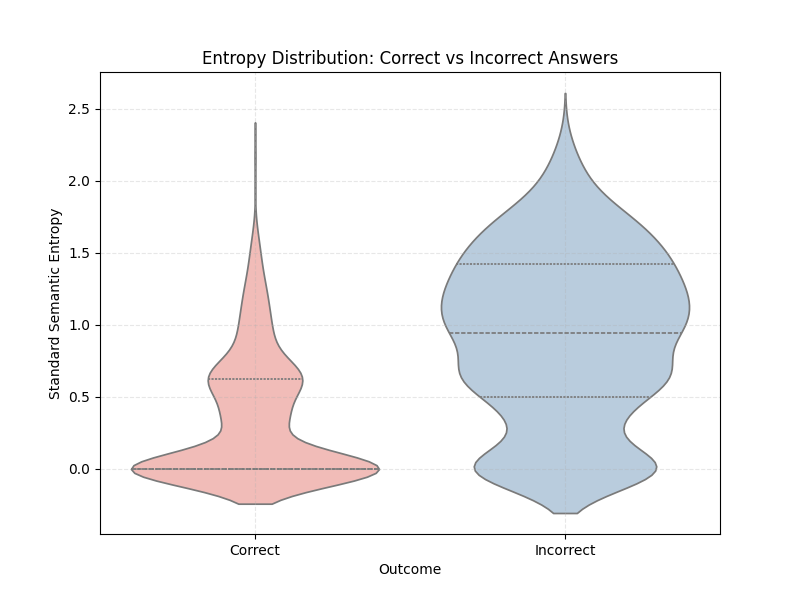
\includegraphics[height=3.5cm, keepaspectratio]{se_correctness_violin.png}
        \caption*{Std SE: Correct vs.\ Incorrect}
    \end{minipage}
    \caption{Distribution of Semantic Entropy across outcomes.}
    \label{fig:se_distributions}
\end{figure*}

\subsection{Additional SE Rejection Curves}

\begin{figure*}[t]
    \centering
    \setlength{\abovecaptionskip}{2pt}
    \begin{minipage}{0.48\textwidth}
        \centering
        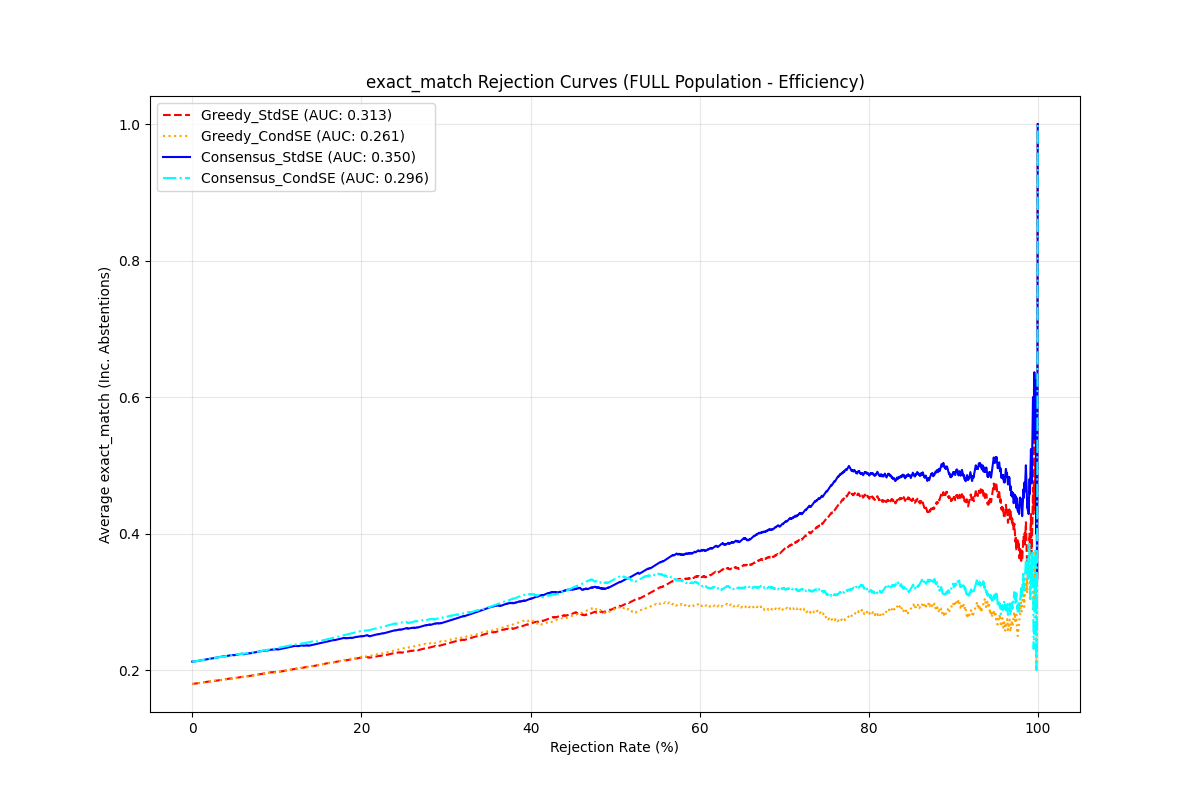
\includegraphics[height=5cm, keepaspectratio]{se_curves_full_exact_match.png}
        \caption*{Full Population (Efficiency)}
    \end{minipage}%
    \hfill
    \begin{minipage}{0.48\textwidth}
        \centering
        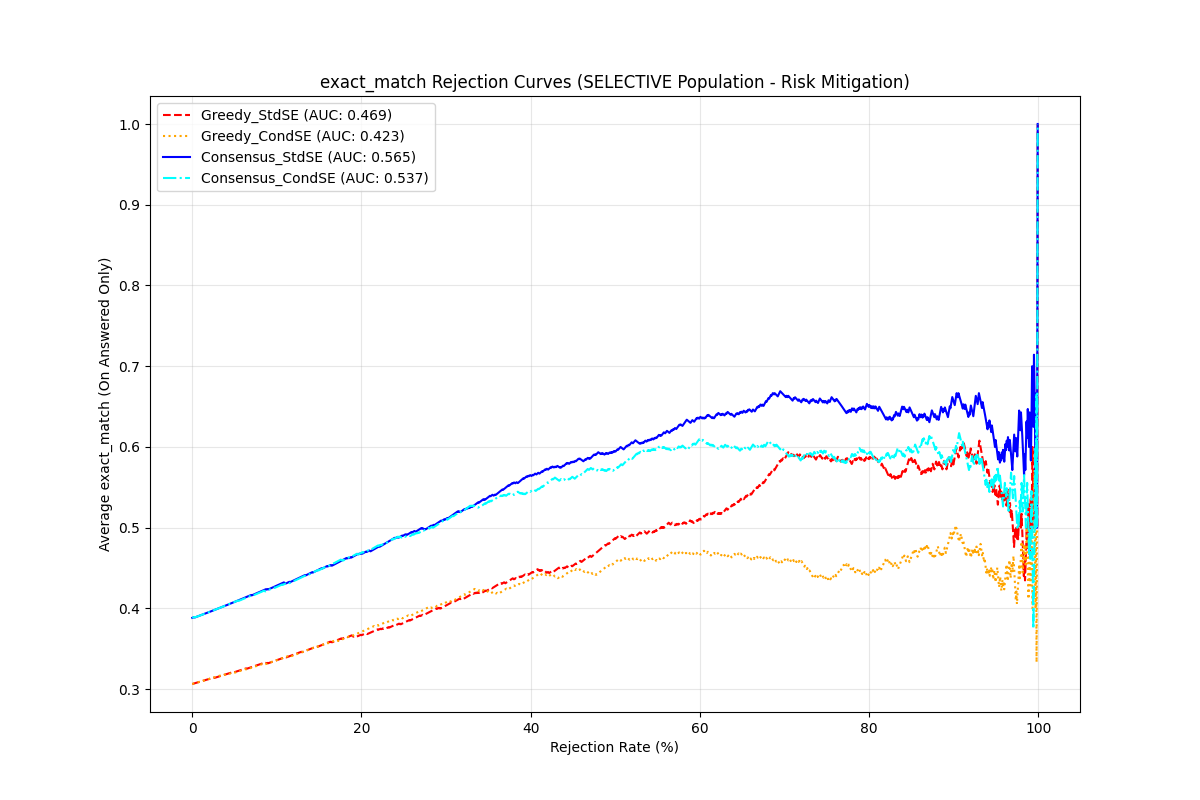
\includegraphics[height=5cm, keepaspectratio]{se_curves_selective_exact_match.png}
        \caption*{Selective Population (Risk Mitigation)}
    \end{minipage}
    \caption{Exact Match (EM) rejection curves.}
    \label{fig:se_em_curves}
\end{figure*}

\begin{table}[H]
\centering
\caption{Impact of Semantic Entropy-based Rejection on Exact Match ($N=2500$)}
\label{tab:se_rejection_em}
\begin{tabular}{llrr}
\toprule
\textbf{Strategy} & \textbf{Rejection Threshold} & \textbf{Full EM} & \textbf{Selective EM} \\
\midrule
Greedy     & 0\%          & 0.1796 & 0.3065 \\
Greedy     & 50\%         & 0.2912 & 0.4863 \\
\midrule
Consensus  & 0\%          & 0.2124 & 0.3884 \\
Consensus  & 50\%         & 0.3256 & \textbf{0.5944} \\
\bottomrule
\end{tabular}
\end{table}

\begin{table}[H]
\centering
\caption{Impact of Semantic Entropy-based Rejection on F1 Scores ($N=2500$)}
\label{tab:se_rejection_f1}
\begin{tabular}{llrr}
\toprule
\textbf{Strategy} & \textbf{Rejection Threshold} & \textbf{Full F1} & \textbf{Selective F1} \\
\midrule
Greedy     & 0\%          & 0.2329 & 0.3974 \\
Greedy     & 50\%         & 0.3482 & 0.5771 \\
\midrule
Consensus  & 0\%          & 0.2719 & 0.4972 \\
Consensus  & 50\%         & 0.3828 & \textbf{0.6991} \\
\bottomrule
\end{tabular}
\end{table}

\subsection{Supplementary RAUQ Rejection Curves}
\begin{figure*}[t]
    \centering
    \begin{minipage}{0.48\textwidth}
        \centering
        \includegraphics[width=\linewidth]{rauq_rejection_curve_vanilla.png}
        \caption*{Vanilla Qwen2.5-7B}
    \end{minipage}%
    \hfill
    \begin{minipage}{0.48\textwidth}
        \centering
        \includegraphics[width=\linewidth]{rauq_rejection_curve_finetuned.png}
        \caption*{Fine-tuned}
    \end{minipage}
    \caption{RAUQ rejection curves: both models improve as high-uncertainty samples are rejected, and the fine-tuned model retains higher quality across the curve.}
    \label{fig:rejection_comparison}
\end{figure*}

\subsection{Confusion Matrices}

\begin{figure*}[t]
    \centering
    \includegraphics[width=\textwidth]{abstention_confusion_matrices_SFT.png}\\[0.2cm]
    \includegraphics[width=\textwidth]{rlhf_confusion_matrices.png}
    \caption{Abstention performance: supervised fine-tuning vs.\ RLVF. \textbf{Top}: confusion matrices for the supervised abstention model (Qwen2.5-Abstain), trained with explicit abstention labels on questions where baseline models failed. \textbf{Bottom}: confusion matrices for the RLVF model, trained with policy-gradient RL against the DeBERTa NLI verifier reward (Section~\ref{sec:rlvf}). Each panel shows how well the model's abstention decisions align with questions that the four reference models answered incorrectly.}
    \label{fig:rlhf_confusion_matrices}
\end{figure*}

\subsection{Additional Tables}

\begin{table}[H]
\centering
\caption{Performance Analysis of Abstention Mechanism Across Reference Models}
\label{tab:abstention_analysis}
\resizebox{\columnwidth}{!}{%
\begin{tabular}{lcccccc}
\toprule
\textbf{Model} & \textbf{Ref. Model} & \textbf{Precision} & \textbf{Recall} & \textbf{TP} & \textbf{FP} & \textbf{FN} \\
 & & & & (Good Abs) & (Bad Abs) & (Missed) \\
\midrule
\multirow{4}{*}{Qwen2.5-Abstain} 
    & Base & \textbf{97.49\%} & 55.69\% & 3,346 & \textbf{86} & 2,662 \\
    & SFT & 95.72\% & 56.83\% & 3,285 & 147 & 2,495 \\
    & CoT & 93.97\% & 57.54\% & 3,225 & 207 & 2,380 \\
    & Hardest & 90.53\% & \textbf{60.85\%} & 3,107 & 325 & \textbf{1,999} \\
\midrule
\multirow{4}{*}{Qwen2.5-RLVF}
    & Base & \textbf{97.84\%} & 49.65\% & 2,983 & \textbf{66} & 3,025 \\
    & SFT & 96.23\% & 50.76\% & 2,934 & 115 & 2,846 \\
    & CoT & 94.19\% & 51.24\% & 2,872 & 177 & 2,733 \\
    & Hardest & 91.21\% & 54.47\% & 2,781 & 268 & 2,325 \\
\bottomrule
\end{tabular}%
}
\end{table}

\begin{table}[h]
\centering
\caption{Overall Model Performance and Error Analysis Relative to Base Model}
\label{tab:model_performance}
\begin{tabular}{lccc}
\toprule
\textbf{Metric} & \textbf{Base Model} & \textbf{SFT Model} & \textbf{CoT Model} \\
\midrule
Overall Accuracy (Exact Match) & 18.87\% & 21.94\% & \textbf{24.31\%} \\
Corrections (Base Wrong $\to$ Right) & -- & 477 & \textbf{697} \\
Regressions (Base Right $\to$ Wrong) & -- & \textbf{249} & 294 \\
\bottomrule
\end{tabular}
\end{table}


\end{document}